
% ----------------------------------------------------------------------
\introduction
\label{sec:intro}
% ----------------------------------------------------------------------

\begin{figure}[t]
	\vspace*{2mm}
	\begin{center}
		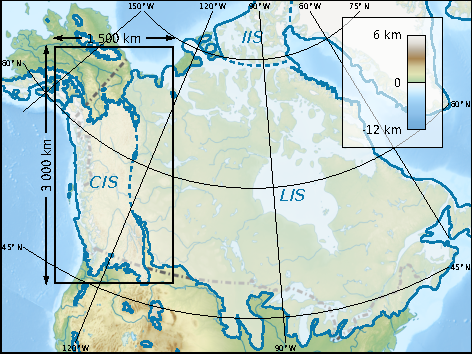
\includegraphics[width=8cm]{cordillera-climate-locmap}
	\end{center}
	\caption{Shaded relief map of northern North America. The frame delimits this study's modelling domain. The outlines of the former ice sheets are from \citet{kleman-etal-2010}. The background map was made with ETOPO1 \citep{data:etopo1} and Natural Earth Data \citep{data:naturalearth}.}
	\label{fig:locmap}
\end{figure}

\emph{Coming soon...}

% Define PISM = Parallel Ice Sheet Model

